\documentclass{standalone}
\usepackage{tikz}
\usetikzlibrary{patterns, positioning}
\usepackage[sfdefault]{ClearSans} %% option 'sfdefault' activates Clear Sans as the default text font
\usepackage[T1]{fontenc}

\begin{document}
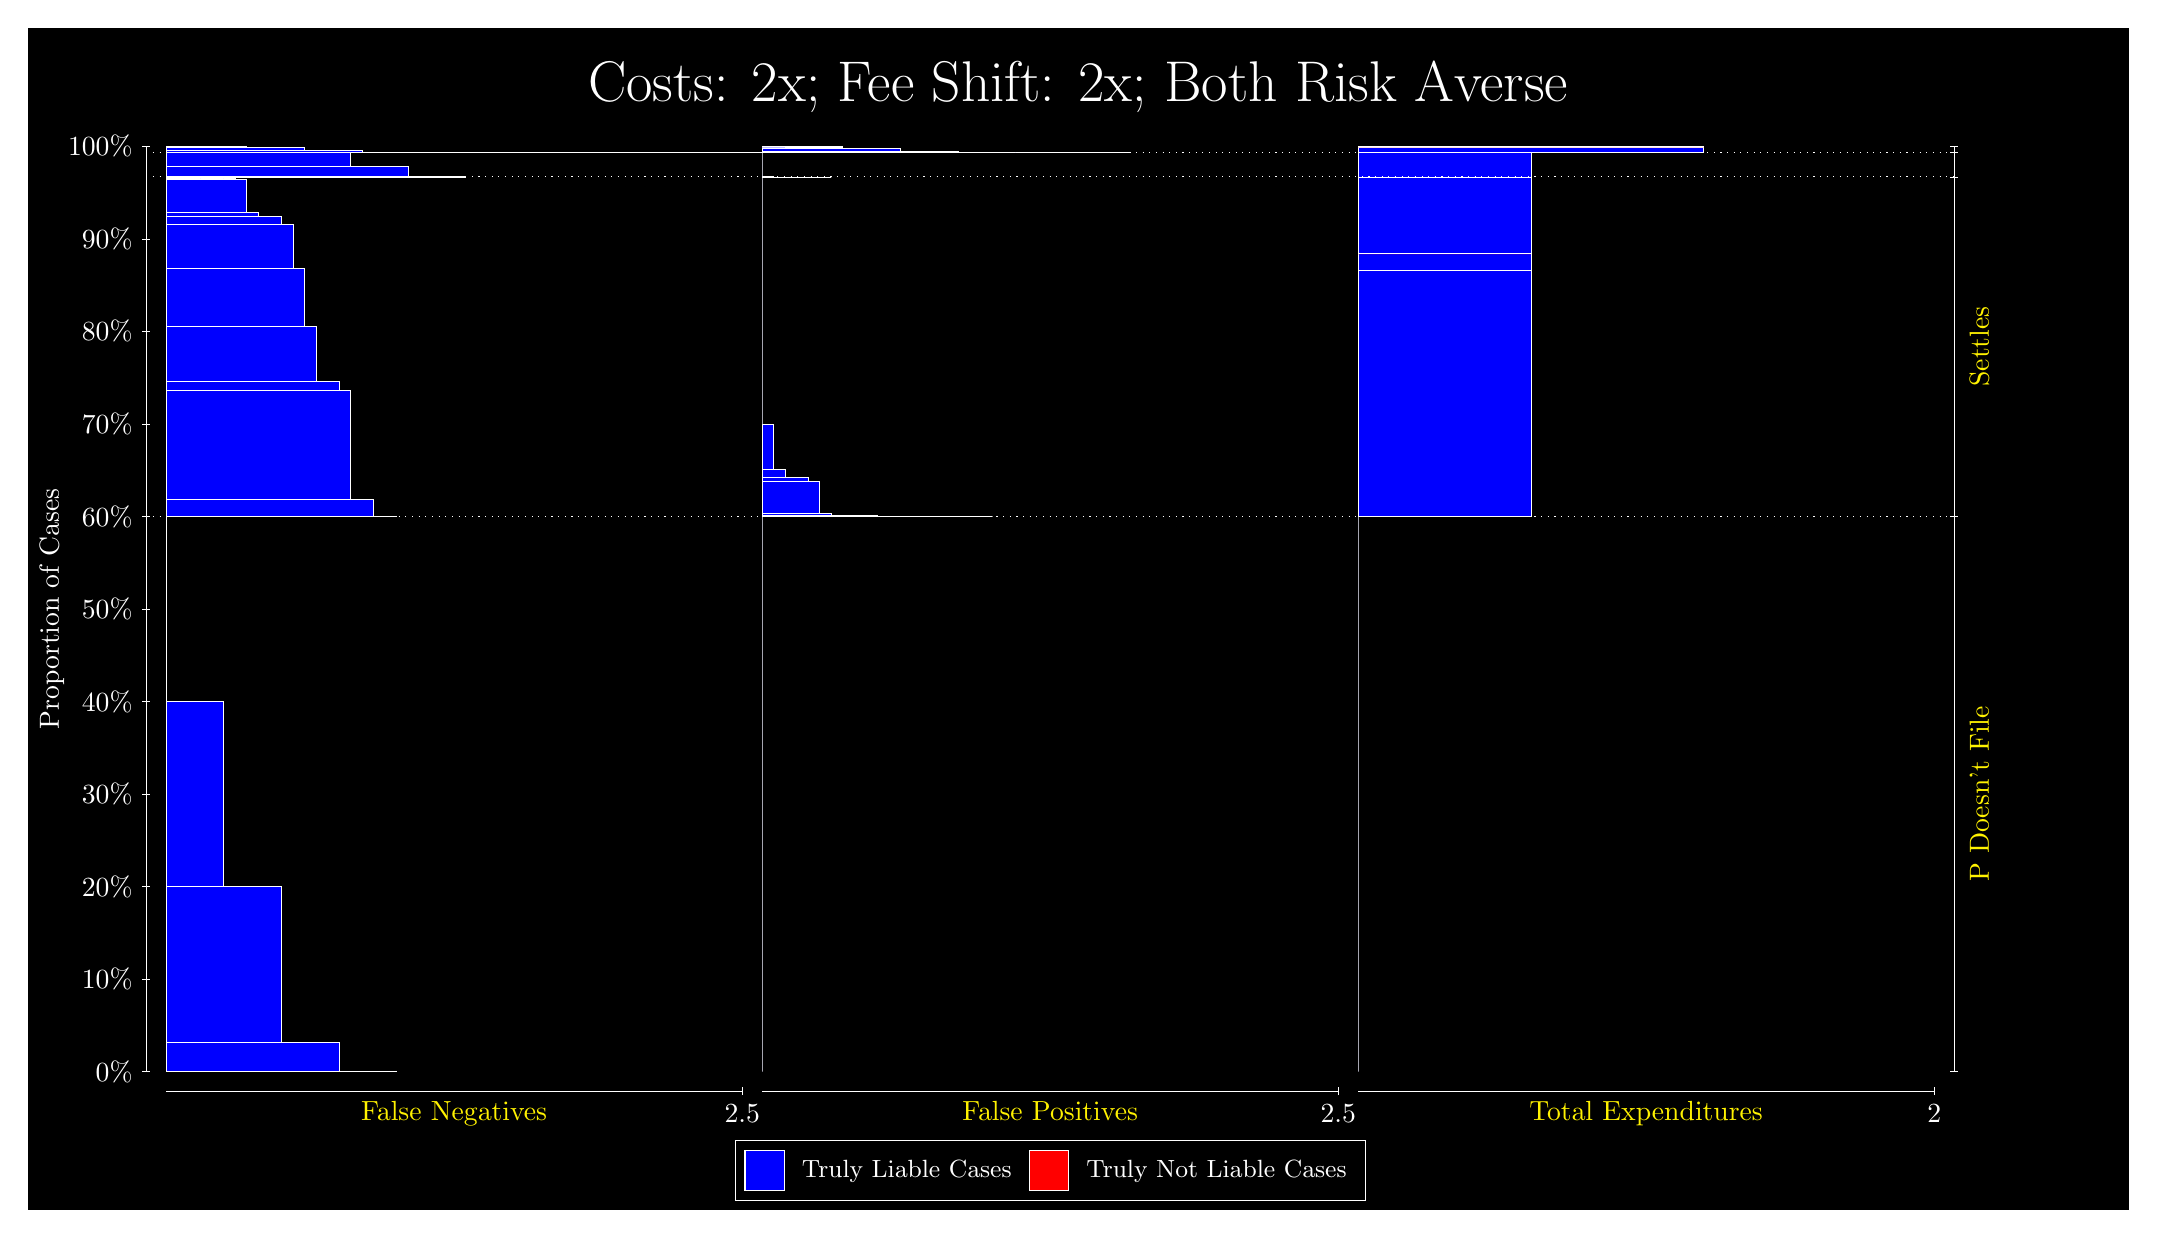
\begin{tikzpicture}
\draw[fill=black] (0,0) rectangle (26.667,15);
\draw[text=white] (0,13.5) rectangle (26.667,15) node[midway] {\huge Costs: 2x; Fee Shift: 2x; Both Risk Averse};
\draw[white, very thin] (1.5,1.75) -- (1.5,13.5);
\node[rotate=90, text=white, anchor=center] at (0.3, 7.625) {Proportion of Cases};
\draw[white, very thin] (1.45,1.75) -- (1.55,1.75);
\node[text=white, anchor=east] at (1.45, 1.75) {0\%};
\draw[white, very thin] (1.45,2.925) -- (1.55,2.925);
\node[text=white, anchor=east] at (1.45, 2.925) {10\%};
\draw[white, very thin] (1.45,4.1) -- (1.55,4.1);
\node[text=white, anchor=east] at (1.45, 4.1) {20\%};
\draw[white, very thin] (1.45,5.275) -- (1.55,5.275);
\node[text=white, anchor=east] at (1.45, 5.275) {30\%};
\draw[white, very thin] (1.45,6.45) -- (1.55,6.45);
\node[text=white, anchor=east] at (1.45, 6.45) {40\%};
\draw[white, very thin] (1.45,7.625) -- (1.55,7.625);
\node[text=white, anchor=east] at (1.45, 7.625) {50\%};
\draw[white, very thin] (1.45,8.8) -- (1.55,8.8);
\node[text=white, anchor=east] at (1.45, 8.8) {60\%};
\draw[white, very thin] (1.45,9.975) -- (1.55,9.975);
\node[text=white, anchor=east] at (1.45, 9.975) {70\%};
\draw[white, very thin] (1.45,11.15) -- (1.55,11.15);
\node[text=white, anchor=east] at (1.45, 11.15) {80\%};
\draw[white, very thin] (1.45,12.325) -- (1.55,12.325);
\node[text=white, anchor=east] at (1.45, 12.325) {90\%};
\draw[white, very thin] (1.45,13.5) -- (1.55,13.5);
\node[text=white, anchor=east] at (1.45, 13.5) {100\%};

\draw[white, very thin] (24.457,1.75) -- (24.457,13.5);
\draw[white, very thin] (24.407,1.75) -- (24.507,1.75);
\node[anchor=west] at (24.407, 1.75) {};
\draw[white, very thin] (24.407,8.8012) -- (24.507,8.8012);
\node[anchor=west] at (24.407, 8.8012) {};
\draw[white, very thin] (24.407,13.112) -- (24.507,13.112);
\node[anchor=west] at (24.407, 13.112) {};
\draw[white, very thin] (24.407,13.424) -- (24.507,13.424);
\node[anchor=west] at (24.407, 13.424) {};
\draw[white, very thin] (24.407,13.5) -- (24.507,13.5);
\node[anchor=west] at (24.407, 13.5) {};

\draw[white, very thin, fill=blue] (1.75,1.75) rectangle (4.6775,1.7538);
\draw[white, very thin, fill=blue] (1.75,1.7538) rectangle (3.9457,2.1271);
\draw[white, very thin, fill=blue] (1.75,2.1271) rectangle (3.2138,4.1043);
\draw[white, very thin, fill=blue] (1.75,4.1043) rectangle (2.4819,6.4512);
\draw[white, very thin, fill=red] (1.75,6.4512) rectangle (1.75,6.4512);
\draw[white, very thin, fill=blue] (1.75,6.4512) rectangle (1.75,8.8012);
\draw[white, very thin, fill=blue] (1.75,8.8012) rectangle (4.6775,8.8015);
\draw[white, very thin, fill=blue] (1.75,8.8015) rectangle (4.3848,9.023);
\draw[white, very thin, fill=blue] (1.75,9.023) rectangle (4.092,10.406);
\draw[white, very thin, fill=blue] (1.75,10.406) rectangle (3.9457,10.51);
\draw[white, very thin, fill=blue] (1.75,10.51) rectangle (3.6529,11.215);
\draw[white, very thin, fill=blue] (1.75,11.215) rectangle (3.5065,11.949);
\draw[white, very thin, fill=blue] (1.75,11.949) rectangle (3.3602,12.513);
\draw[white, very thin, fill=blue] (1.75,12.513) rectangle (3.2138,12.617);
\draw[white, very thin, fill=blue] (1.75,12.617) rectangle (2.921,12.667);
\draw[white, very thin, fill=blue] (1.75,12.667) rectangle (2.7746,13.078);
\draw[white, very thin, fill=blue] (1.75,13.078) rectangle (2.6283,13.099);
\draw[white, very thin, fill=blue] (1.75,13.099) rectangle (2.4819,13.099);
\draw[white, very thin, fill=blue] (1.75,13.099) rectangle (2.1891,13.099);
\draw[white, very thin, fill=blue] (1.75,13.099) rectangle (2.0428,13.112);
\draw[white, very thin, fill=blue] (1.75,13.112) rectangle (1.8964,13.112);
\draw[white, very thin, fill=red] (1.75,13.112) rectangle (1.75,13.112);
\draw[white, very thin, fill=blue] (1.75,13.112) rectangle (1.75,13.112);
\draw[white, very thin, fill=blue] (1.75,13.112) rectangle (5.5558,13.114);
\draw[white, very thin, fill=blue] (1.75,13.114) rectangle (4.8239,13.248);
\draw[white, very thin, fill=blue] (1.75,13.248) rectangle (4.092,13.422);
\draw[white, very thin, fill=blue] (1.75,13.422) rectangle (3.3602,13.424);
\draw[white, very thin, fill=blue] (1.75,13.424) rectangle (2.6283,13.424);
\draw[white, very thin, fill=red] (1.75,13.424) rectangle (1.75,13.424);
\draw[white, very thin, fill=blue] (1.75,13.424) rectangle (9.9471,13.424);
\draw[white, very thin, fill=blue] (1.75,13.424) rectangle (9.2152,13.424);
\draw[white, very thin, fill=blue] (1.75,13.424) rectangle (8.4834,13.426);
\draw[white, very thin, fill=blue] (1.75,13.426) rectangle (7.7515,13.427);
\draw[white, very thin, fill=blue] (1.75,13.427) rectangle (7.0196,13.427);
\draw[white, very thin, fill=blue] (1.75,13.427) rectangle (6.2877,13.427);
\draw[white, very thin, fill=blue] (1.75,13.427) rectangle (5.7022,13.427);
\draw[white, very thin, fill=blue] (1.75,13.427) rectangle (5.5558,13.427);
\draw[white, very thin, fill=blue] (1.75,13.427) rectangle (4.9703,13.428);
\draw[white, very thin, fill=blue] (1.75,13.428) rectangle (4.2384,13.444);
\draw[white, very thin, fill=blue] (1.75,13.444) rectangle (3.5065,13.484);
\draw[white, very thin, fill=blue] (1.75,13.484) rectangle (2.7746,13.5);
\draw[white, very thin, fill=blue] (1.75,13.5) rectangle (2.0428,13.5);
\draw[white, very thin, fill=red] (1.75,13.5) rectangle (1.75,13.5);
\draw[white, very thin, fill=blue] (1.75,13.5) rectangle (1.75,13.5);
\draw[white, very thin, fill=red] (9.3189,1.75) rectangle (9.3189,1.75);
\draw[white, very thin, fill=blue] (9.3189,1.75) rectangle (9.3189,8.8012);
\draw[white, very thin, fill=red] (9.3189,8.8012) rectangle (12.246,8.8012);
\draw[white, very thin, fill=blue] (9.3189,8.8012) rectangle (12.246,8.8012);
\draw[white, very thin, fill=red] (9.3189,8.8012) rectangle (11.661,8.8012);
\draw[white, very thin, fill=blue] (9.3189,8.8012) rectangle (11.661,8.8012);
\draw[white, very thin, fill=blue] (9.3189,8.8012) rectangle (11.515,8.8012);
\draw[white, very thin, fill=red] (9.3189,8.8012) rectangle (11.368,8.8012);
\draw[white, very thin, fill=blue] (9.3189,8.8012) rectangle (11.368,8.8012);
\draw[white, very thin, fill=red] (9.3189,8.8012) rectangle (11.075,8.8012);
\draw[white, very thin, fill=blue] (9.3189,8.8012) rectangle (11.075,8.8012);
\draw[white, very thin, fill=blue] (9.3189,8.8012) rectangle (10.929,8.8012);
\draw[white, very thin, fill=blue] (9.3189,8.8012) rectangle (10.783,8.8147);
\draw[white, very thin, fill=blue] (9.3189,8.8147) rectangle (10.636,8.8148);
\draw[white, very thin, fill=blue] (9.3189,8.8148) rectangle (10.344,8.815);
\draw[white, very thin, fill=blue] (9.3189,8.815) rectangle (10.197,8.836);
\draw[white, very thin, fill=blue] (9.3189,8.836) rectangle (10.051,9.2467);
\draw[white, very thin, fill=blue] (9.3189,9.2467) rectangle (9.9044,9.2964);
\draw[white, very thin, fill=blue] (9.3189,9.2964) rectangle (9.6116,9.4005);
\draw[white, very thin, fill=blue] (9.3189,9.4005) rectangle (9.4652,9.9651);
\draw[white, very thin, fill=blue] (9.3189,9.9651) rectangle (9.3189,13.112);
\draw[white, very thin, fill=red] (9.3189,13.112) rectangle (10.197,13.112);
\draw[white, very thin, fill=blue] (9.3189,13.112) rectangle (10.197,13.112);
\draw[white, very thin, fill=blue] (9.3189,13.112) rectangle (9.4652,13.115);
\draw[white, very thin, fill=blue] (9.3189,13.115) rectangle (9.3189,13.424);
\draw[white, very thin, fill=red] (9.3189,13.424) rectangle (14.003,13.424);
\draw[white, very thin, fill=blue] (9.3189,13.424) rectangle (14.003,13.424);
\draw[white, very thin, fill=red] (9.3189,13.424) rectangle (13.271,13.424);
\draw[white, very thin, fill=blue] (9.3189,13.424) rectangle (13.271,13.424);
\draw[white, very thin, fill=red] (9.3189,13.424) rectangle (12.539,13.424);
\draw[white, very thin, fill=blue] (9.3189,13.424) rectangle (12.539,13.424);
\draw[white, very thin, fill=blue] (9.3189,13.424) rectangle (11.807,13.441);
\draw[white, very thin, fill=red] (9.3189,13.441) rectangle (11.807,13.441);
\draw[white, very thin, fill=blue] (9.3189,13.441) rectangle (11.807,13.441);
\draw[white, very thin, fill=blue] (9.3189,13.441) rectangle (11.075,13.48);
\draw[white, very thin, fill=blue] (9.3189,13.48) rectangle (11.075,13.48);
\draw[white, very thin, fill=blue] (9.3189,13.48) rectangle (10.344,13.494);
\draw[white, very thin, fill=blue] (9.3189,13.494) rectangle (10.344,13.497);
\draw[white, very thin, fill=blue] (9.3189,13.497) rectangle (9.6116,13.497);
\draw[white, very thin, fill=blue] (9.3189,13.497) rectangle (9.6116,13.497);
\draw[white, very thin, fill=red] (9.3189,13.497) rectangle (9.3189,13.497);
\draw[white, very thin, fill=blue] (9.3189,13.497) rectangle (9.3189,13.5);
\draw[white, very thin, fill=red] (16.888,1.75) rectangle (16.888,1.75);
\draw[white, very thin, fill=blue] (16.888,1.75) rectangle (16.888,8.8012);
\draw[white, very thin, fill=red] (16.888,8.8012) rectangle (19.083,8.8012);
\draw[white, very thin, fill=blue] (16.888,8.8012) rectangle (19.083,11.927);
\draw[white, very thin, fill=red] (16.888,11.927) rectangle (19.083,11.927);
\draw[white, very thin, fill=blue] (16.888,11.927) rectangle (19.083,12.136);
\draw[white, very thin, fill=red] (16.888,12.136) rectangle (19.083,12.136);
\draw[white, very thin, fill=blue] (16.888,12.136) rectangle (19.083,13.112);
\draw[white, very thin, fill=red] (16.888,13.112) rectangle (19.083,13.112);
\draw[white, very thin, fill=blue] (16.888,13.112) rectangle (19.083,13.424);
\draw[white, very thin, fill=red] (16.888,13.424) rectangle (21.279,13.424);
\draw[white, very thin, fill=blue] (16.888,13.424) rectangle (21.279,13.494);
\draw[white, very thin, fill=red] (16.888,13.494) rectangle (21.279,13.494);
\draw[white, very thin, fill=blue] (16.888,13.494) rectangle (21.279,13.497);
\draw[white, very thin, fill=red] (16.888,13.497) rectangle (21.279,13.497);
\draw[white, very thin, fill=blue] (16.888,13.497) rectangle (21.279,13.5);
\draw[white, dotted] (1.5,8.8012) -- (24.457,8.8012);
\draw[white, dotted] (1.5,13.112) -- (24.457,13.112);
\draw[white, dotted] (1.5,13.424) -- (24.457,13.424);
\draw[white, very thin] (1.75,1.5) -- (9.0689,1.5);
\node[text=yellow, anchor=north] at (5.4094, 1.5) {False Negatives};
\draw[white, very thin] (9.0689,1.45) -- (9.0689,1.55);
\node[text=white, anchor=north] at (9.0689, 1.45) {2.5};

\draw[white, very thin] (9.3189,1.5) -- (16.638,1.5);
\node[text=yellow, anchor=north] at (12.978, 1.5) {False Positives};
\draw[white, very thin] (16.638,1.45) -- (16.638,1.55);
\node[text=white, anchor=north] at (16.638, 1.45) {2.5};

\draw[white, very thin] (16.888,1.5) -- (24.207,1.5);
\node[text=yellow, anchor=north] at (20.547, 1.5) {Total Expenditures};
\draw[white, very thin] (24.207,1.45) -- (24.207,1.55);
\node[text=white, anchor=north] at (24.207, 1.45) {2};

\node[text=yellow, centered, rotate=90] at (24.777, 5.2756) {P Doesn't File};
\node[text=yellow, centered, rotate=90] at (24.777, 10.957) {Settles};



\draw (12.978300999999998,1.5) node[draw=none] (baseCoordinate) {};
\begin{scope}[align=center]
        \matrix[scale=0.5, draw=white, below=0.5cm of baseCoordinate, nodes={draw}, column sep=0.1cm]{
            \node[rectangle, draw, minimum width=0.5cm, minimum height=0.5cm, fill=blue] {}; &
            \node[draw=none, font=\small, text=white] (B) {Truly Liable Cases}; &
            \node[rectangle, draw, minimum width=0.5cm, minimum height=0.5cm, fill=red] {}; &
            \node[draw=none, font=\small, text=white] (B) {Truly Not Liable Cases}; \\
            };
\end{scope}

\end{tikzpicture}
\end{document}